\documentclass[11pt]{scrartcl}

\usepackage{ucs}
\usepackage[utf8x]{inputenc}
\usepackage{ngerman}
\usepackage{amsmath,amssymb,amstext}
\usepackage{graphicx}
\usepackage[automark]{scrpage2}
\usepackage{pgfplots}
\usepackage{chngcntr}
\usepackage[left=3cm, right=3cm, top=3cm, bottom=3cm]{geometry}
\counterwithin{figure}{section}

\pagestyle{scrheadings}

\title{Hybrid-Quicksort}
\author{Finn Jannsen, Philipp Schwarz}
\date{\today{}}

\begin{document}

\maketitle

\tableofcontents

\section{Einführung}
	\label{sec:einfuehrung}
	
	Diese Dokumentation beschreibt eine Sortieralgorithmus-Implementation für Arrays, basierend auf Quicksort.
	Für den Algorithmus wurden Optimierungen ausgeführt, die reduzierte Laufzeit und effiziente Resourcennutzung zum Ziel haben.
	In Abschnitt \ref{sec:implementation} wird darauf eingegangen, wie der Algorithmus realisiert wurde.
	Anschließend wird in Abschnitt \ref{sec:veri} geprüft, ob die Implementation korrekt funktioniert 
	und in Abschnitt \ref{sec:aufwand} die Performance mit dem zu Grunde liegenden Quicksort verglichen.

\section{Implementation}
	\label{sec:implementation}
	
	Der Algorithmus wurde als Kasse realisiert, der ein Interface implementiert, welches es ermöglicht, einfach weitere Implementationen, sofern dies gewünscht wird, zu schreiben.

	\subsection{Pivotauswahl}
		\label{sec:pivAus}
		
		Bei der Untersuchung von Quicksort stellte sich eine Methode zur Pivot-Auswahl am effizientesten auf: Median-of-three.
		Der mittlere Wert von mehreren Key-Werten (bei Bedarf auch von mehr als 3) sorgt für eine gleichmäßigere Aufteilung der Partitionierung beim Sortieren.
		Dadurch finden im allgemeinen weniger Iterationen als bei anderen Pivots, wie z.B. Random oder Right statt, was wünschenswert ist.
 
		Der Code ist in \ref{figure:pivotCode} dargestellt. Eins von 3 Elementen wird in die Mitte getauscht und als Pivot ausgewählt.
	
	\subsection{Sortieren}
		\label{sec:sortAlgo}
		
		Der bisherige Quicksort-Algorithmus besteht im wesentlichen aus einer Schleife, in der zuerst das erste Element von links, welches gleich oder größer als Pivot ist, gesucht wird.
		Danach wird das erste Element von rechts, welches kleiner als das Pivot ist, gesucht. Diese werden dann getauscht.
		Die Schleife wird verlassen, wenn die jeweiligen Such-Schleifen einander kreuzen.
		Danach wird das Pivot in diese Mitte an Stelle i zurückgetauscht und der Algorithmus wird zwei mal rekursiv gestartet,
		einmal um die Liste von ganz links bis i-1 zu sortieren und noch einmal um die Liste von i+1 bis rechts zu sortieren.

		Für dieses Hybrid-Quicksort wurde eine Implementation von Quicksort mit Partitionierung in 3 Teile ausgewählt.
		Das Pivot steht hier anfänglich links. Nun wird der Array von einer Seite an durchiteriert.
		Ist ein Element kleiner, so wird es nach links getauscht und ein Counter erhöht, sodass das nächste kleinere Element daneben platziert würde.
		Ist ein Element größer, wird es nach rechts getauscht und ein Counter verringert, um das nächste größere Element daneben zu platzieren.
		Wenn es gleich dem Pivot ist, so bleibt es stehen. 
		Dadurch überspringt man redundantes Tauschen duplizierter Elemente und durch das Tauschen kleinerer Elemente wird das Pivot automatisch immer wieder in die Mitte getauscht.
		Danach wird wieder mit den linken und rechten Teilen des Pivots rekursiv sortiert.

		Der Code hierfür ist in \ref{figure:sortCode} dargestellt.

	\subsection{Optimierung}
		\label{sec:optAlgo}

		Der Algorithmus wurde weiterhin mit Insertionsort bei einer Anzahl an Elementen kleiner als 10 optimiert.
		Durch diese Praxis wird ein hoher Overhead bei kleinen Arrays durch die rekursiven Aufrufe verhindert.
		In der Praxis wurden verschiedene Werte für die für den Aufruf von Insertionsort benötigte Anzahl an Elementen getestet,
		sowohl mit sehr vielen Duplikaten (Begrenzung der Keys auf 100 Werte), als auch mit wenigen.
		Dies ist zu sehen in Abbildung \ref{figure:table}. 
		Mit einer Versuchsgröße von 100 zeigt ein recht genauer Durchschnittswert eine eindeutige Verbesserung der Performance mit 10 Insertions.

\section{Testen und Verifikation}
\label{sec:vertests}

	\subsection{Verifizieren}
		\label{sec:veri}
		
		Der Algorithmus wurde auf seine korrekte Funktionalität getestet.
		Hierzu zählt natürlich das Vorliegen des Ergebnisses in der korrekten Reihenfolge.
		Alle Tests wurden erfolgreich mit unterschiedlichen Eingabewerten absolviert.
	
	\subsection{Aufwandsanalyse}
		\label{sec:aufwand}
		
		Für die Aufwandsanalyse wurde der Klasse ein Counter eingeführt, der die Tauschoperationen zählt, als auch die Ausführungszeit beobachtet. 
		
		Bisherige Untersuchungen von Quicksort haben bereits einen Asymptotischen Aufwand wie folgt ergeben:

		Rechenoperationen bei Best- und Average Case:
		\begin{equation*}
		T(n) = \mathcal{O}(n*ln(n))
		\end{equation*}
		Rechenoperationen bei Worst Case:
		\begin{equation*}
		T(n) = \mathcal{O}(n^{2})
		\end{equation*}

		Da sich der Rechenaufwand für Worst Case bei unserer Implementation sich nicht ändert 
		und dieser auch besonders selten ist, wurden dieses mal zufällig Sortierte Arrays beobachtet.
		Außerdem wurden dieses mal statt komplett zufälligen Key-Werten welche mit folgender Beschränkung ausgewählt: 
		\begin{equation*}
		700*N \leq key \leq 800*N
		\end{equation*}
		Dies hat zur Folge, dass in der zu sortierenden Menge vermehrt duplizierte Keys auftreten. 
		Um unter anderem mit dieser Hürde besser umgehen zu können wurden die in \ref{sec:optAlgo} angesprochenen Optimierungen eingeführt.
		Es wurden 100 Durchläufe des Tests mit den Größen $N=10^k, k=1,...,6$ durchgeführt, um einen angemessenen Mittelwert zu ermitteln.

		Es wurden zuerst viele einzigartige Keys verwendet, um die allgemeine Performance zu vergleichen.
		Die Ergebnisse für die Rechenoperationen sind in Abbildung \ref{figure:ranOperTest}, für die Laufzeit in \ref{figure:ranTimeTest} zu sehen.
		Es ist ersichtlich, dass das Hybrid-Quicksort womöglich durch Insertionsort eine wenig höhere Anzahl an Rechenoperationen hat, dafür aber einen zeitlichen Vorteil erzielt.
		Dies liegt an der effizienteren Nutzung der Resourcen.

		Diese Versuche wurden auch für eine vermehrte Anzahl an Duplikaten (max. 100 eindeutige keys) durchgeführt, 
		was zeigt, wie effizient Hybrid-Quicksort im Gegensatz zu normalem Quicksort mit dieser Hürde umgehen kann.
		Die Ergebnisse sind in Abbildung \ref{figure:dupOperTest} und \ref{figure:dupTimeTest} zu sehen.

\begin{figure}
    \newcommand{\fqsCol}{blue}
    \newcommand{\qsCol}{red}
    \newcommand{\bestAvgMark}{square*}
    \newcommand{\transparent}{0.8}
    \makebox[\textwidth][c]{
    \begin{tikzpicture}
        \begin{loglogaxis}[
                title={\large Berechnung Operationen},
                height=10cm,
                width=17cm,
                grid=major,
                x tick label style={
                /pgf/number format/1000 sep=},
                ylabel=Operationen,
                xlabel=Anzahl Elemente,
                enlargelimits=0.05,
                legend style={at={(0.5,-0.15)},
                anchor=north,legend columns=1},
            ]
            \addplot[color=\fqsCol,mark=\bestAvgMark,opacity=\transparent]
                coordinates {(1,0)(10,21.41)(100,573.08)(1000,9568.58)(10000,135268.23)(100000,1741991.22)(1000000,21407968.93)};
            \addplot[color=\qsCol,mark=\bestAvgMark,opacity=\transparent]
                coordinates {(1,0)(10,21.05)(100,562.34)(1000,9445.31)(10000,133652.47)(100000,1731953.94)(1000000,21272971.31)};
            \legend{Hybrid-Quicksort, Quicksort}
        \end{loglogaxis}
    \end{tikzpicture}
    }
    \caption{Quantitativer Vergleich zu Quicksort anhand Rechenoperationen}
    \label{figure:ranOperTest}
\end{figure}


\begin{figure}
    \newcommand{\fqsCol}{blue}
    \newcommand{\qsCol}{red}
    \newcommand{\bestAvgMark}{square*}
    \newcommand{\transparent}{0.8}
    \makebox[\textwidth][c]{
    \begin{tikzpicture}
        \begin{loglogaxis}[
                title={\large Berechnung Operationen},
                height=10cm,
                width=17cm,
                grid=major,
                x tick label style={
                /pgf/number format/1000 sep=},
                ylabel=Zeit in ms,
                xlabel=Anzahl Elemente,
                enlargelimits=0.05,
                legend style={at={(0.5,-0.15)},
                anchor=north,legend columns=1},
            ]
            \addplot[color=\fqsCol,mark=\bestAvgMark,opacity=\transparent]
                coordinates {(1,0)(10,0)(100,0.01)(1000,0.1)(10000,1.25)(100000,19.09)(1000000,340.34)};
            \addplot[color=\qsCol,mark=\bestAvgMark,opacity=\transparent]
                coordinates {(1,0)(10,0)(100,0)(1000,0.12)(10000,1.36)(100000,20.5)(1000000,350.09)};
            \legend{Hybrid-Quicksort, Quicksort}
        \end{loglogaxis}
    \end{tikzpicture}
    }
    \caption{Quantitativer Vergleich zu Quicksort anhand Laufzeit}
    \label{figure:ranTimeTest}
\end{figure}

\begin{figure}
    \newcommand{\fqsCol}{blue}
    \newcommand{\qsCol}{red}
    \newcommand{\bestAvgMark}{square*}
    \newcommand{\transparent}{0.8}
    \makebox[\textwidth][c]{
    \begin{tikzpicture}
        \begin{loglogaxis}[
                title={\large Berechnung Operationen},
                height=10cm,
                width=17cm,
                grid=major,
                x tick label style={
                /pgf/number format/1000 sep=},
                ylabel=Operationen,
                xlabel=Anzahl Elemente,
                enlargelimits=0.05,
                legend style={at={(0.5,-0.15)},
                anchor=north,legend columns=1},
            ]
            \addplot[color=\fqsCol,mark=\bestAvgMark,opacity=\transparent]
                coordinates {(1,0)(10,23.9)(100,524.5)(1000,6361.6)(10000,69383.6)(100000,670892)(1000000,6565845)};
            \addplot[color=\qsCol,mark=\bestAvgMark,opacity=\transparent]
                coordinates {(1,0)(10,21.6)(100,574.7)(1000,11318.9)(10000,569145.2)(100000,50659668.7)(1000000,5006527795)};
            \legend{Hybrid-Quicksort, Quicksort}
        \end{loglogaxis}
    \end{tikzpicture}
    }
    \caption{Quantitativer Vergleich zu Quicksort anhand Rechenoperationen mit vermehrten Duplikaten}
    \label{figure:dupOperTest}
\end{figure}


\begin{figure}
    \newcommand{\fqsCol}{blue}
    \newcommand{\qsCol}{red}
    \newcommand{\bestAvgMark}{square*}
    \newcommand{\transparent}{0.8}
    \makebox[\textwidth][c]{
    \begin{tikzpicture}
        \begin{loglogaxis}[
                title={\large Berechnung Operationen},
                height=10cm,
                width=17cm,
                grid=major,
                x tick label style={
                /pgf/number format/1000 sep=},
                ylabel=Zeit in ms,
                xlabel=Anzahl Elemente,
                enlargelimits=0.05,
                legend style={at={(0.5,-0.15)},
                anchor=north,legend columns=1},
            ]
            \addplot[color=\fqsCol,mark=\bestAvgMark,opacity=\transparent]
                coordinates {(1,0)(10,0)(100,0)(1000,0)(10000,0.7)(100000,8.8)(1000000,156.6)};
            \addplot[color=\qsCol,mark=\bestAvgMark,opacity=\transparent]
                coordinates {(1,0)(10,0.1)(100,0.1)(1000,0.4)(10000,2.1)(100000,147.2)(1000000,21161.5)};
            \legend{Hybrid-Quicksort, Quicksort}
        \end{loglogaxis}
    \end{tikzpicture}
    }
    \caption{Quantitativer Vergleich zu Quicksort anhand Laufzeit mit vermehrten Duplikaten}
    \label{figure:dupTimeTest}
\end{figure}

\begin{figure}
\begin{verbatim}
//find pivot with median of 3
int center = (left + right) / 2;

if (list[left].getKey() > list[center].getKey()) {
    increaseCounter();
    swap(list, left, center);
}
if (list[left].getKey() > list[right].getKey()) {
    increaseCounter();
    swap(list, left, right);
}
if (list[center].getKey() > list[right].getKey()) {
    increaseCounter();
    swap(list, center, right);
}
\end{verbatim}
\caption{Code-Ausschnitt Pivotsuche}
\label{figure:pivotCode}
\end{figure}


\begin{figure}
\begin{verbatim}
int low = left, high = right;
int pivot = list[left].getKey();
int i = left;

while (true) {
    if (list[i].getKey() < pivot) {
        // smaller than pivot, accumulate from the left and eventually shift pivot to i
        swap(list, i, low);
        i++; 
        low++;
        Counter++;
    } else if (list[i].getKey() > pivot) {
        // bigger than pivot, accumulate from the right
        swap(list, i, high);
        high--;
        Counter++;
    } else {
        // ran over pivot, skip
        i++;
        Counter++;
    }
    if (i > high) {
        // don't run over already iterated elements
        break;
    }
}
\end{verbatim}
\caption{Code-Ausschnitt Sortieren}
\label{figure:sortCode}
\end{figure}

\begin{figure}
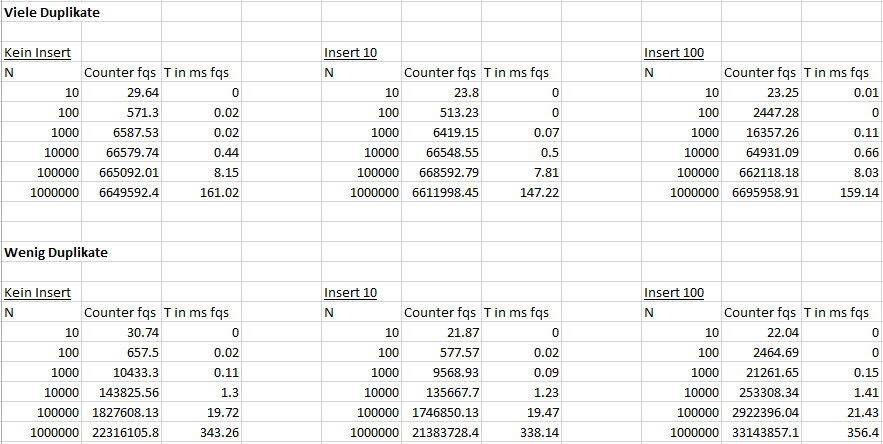
\includegraphics[width=\linewidth]{insertiontable.png}
\caption{Durchschnittswerte unterschiedlicher Insertionsorts von 100 Durchführungen bei vielen und wenigen Duplikaten}
\label{figure:table}
\end{figure}
\end{document}